% UFRN - CT - DCA
% Controle Avançado - Lista 1
% Questão 2
% Autor: Cristiano Gurgel de Castro <crisgc@dca.ufrn.br>

\section*{Questão 2}

\textit{Um sistema com realimentação unitária tem a seguinte função de
transferência de malha aberta:}

\begin{flalign*}
G(s) = \frac{s+r}{(s+p)(s+q)}
\end{flalign*}

\noindent \textit{em que $0 \leq p \leq 5$, $0 \leq q \leq 1$ e $1 \leq r \leq
2$.  Selecione os parâmetros (todos reais) de um controlador atraso-avanço de
fase, de forma que o sistema em malha fechada tenha um desempenho robusto. Faça
simulações no \emph{Matlab} para comprovar o desempenho do sistema.}

\vspace{0.5cm}

\noindent{\bf Resolução:}

\vspace{0.25cm}

Para efeitos de análise e projeto dos controladores, utilizamos os valores médio
de cada um dos parâmetros, a saber $\vmedio{r} = 1,5$, $\vmedio{p} = 4$ e
$\vmedio{q} = 0,5$ e a função de transferência de malha aberta é escrita como

\begin{flalign}
\vmedio{G}(s) & = \frac{s+\vmedio{r}}{(s+\vmedio{p})(s+\vmedio{q})}  =
\frac{s+1,5}{(s+4)(s+0,5)} = {\frac{1,5+s}{2+4,5s+s^{2}}} \label{eq:q2:gma}
\end{flalign}

\noindent e o lugar das raízes para esse sistema é mostrado a seguir:

\begin{figure}[htb]
\centering
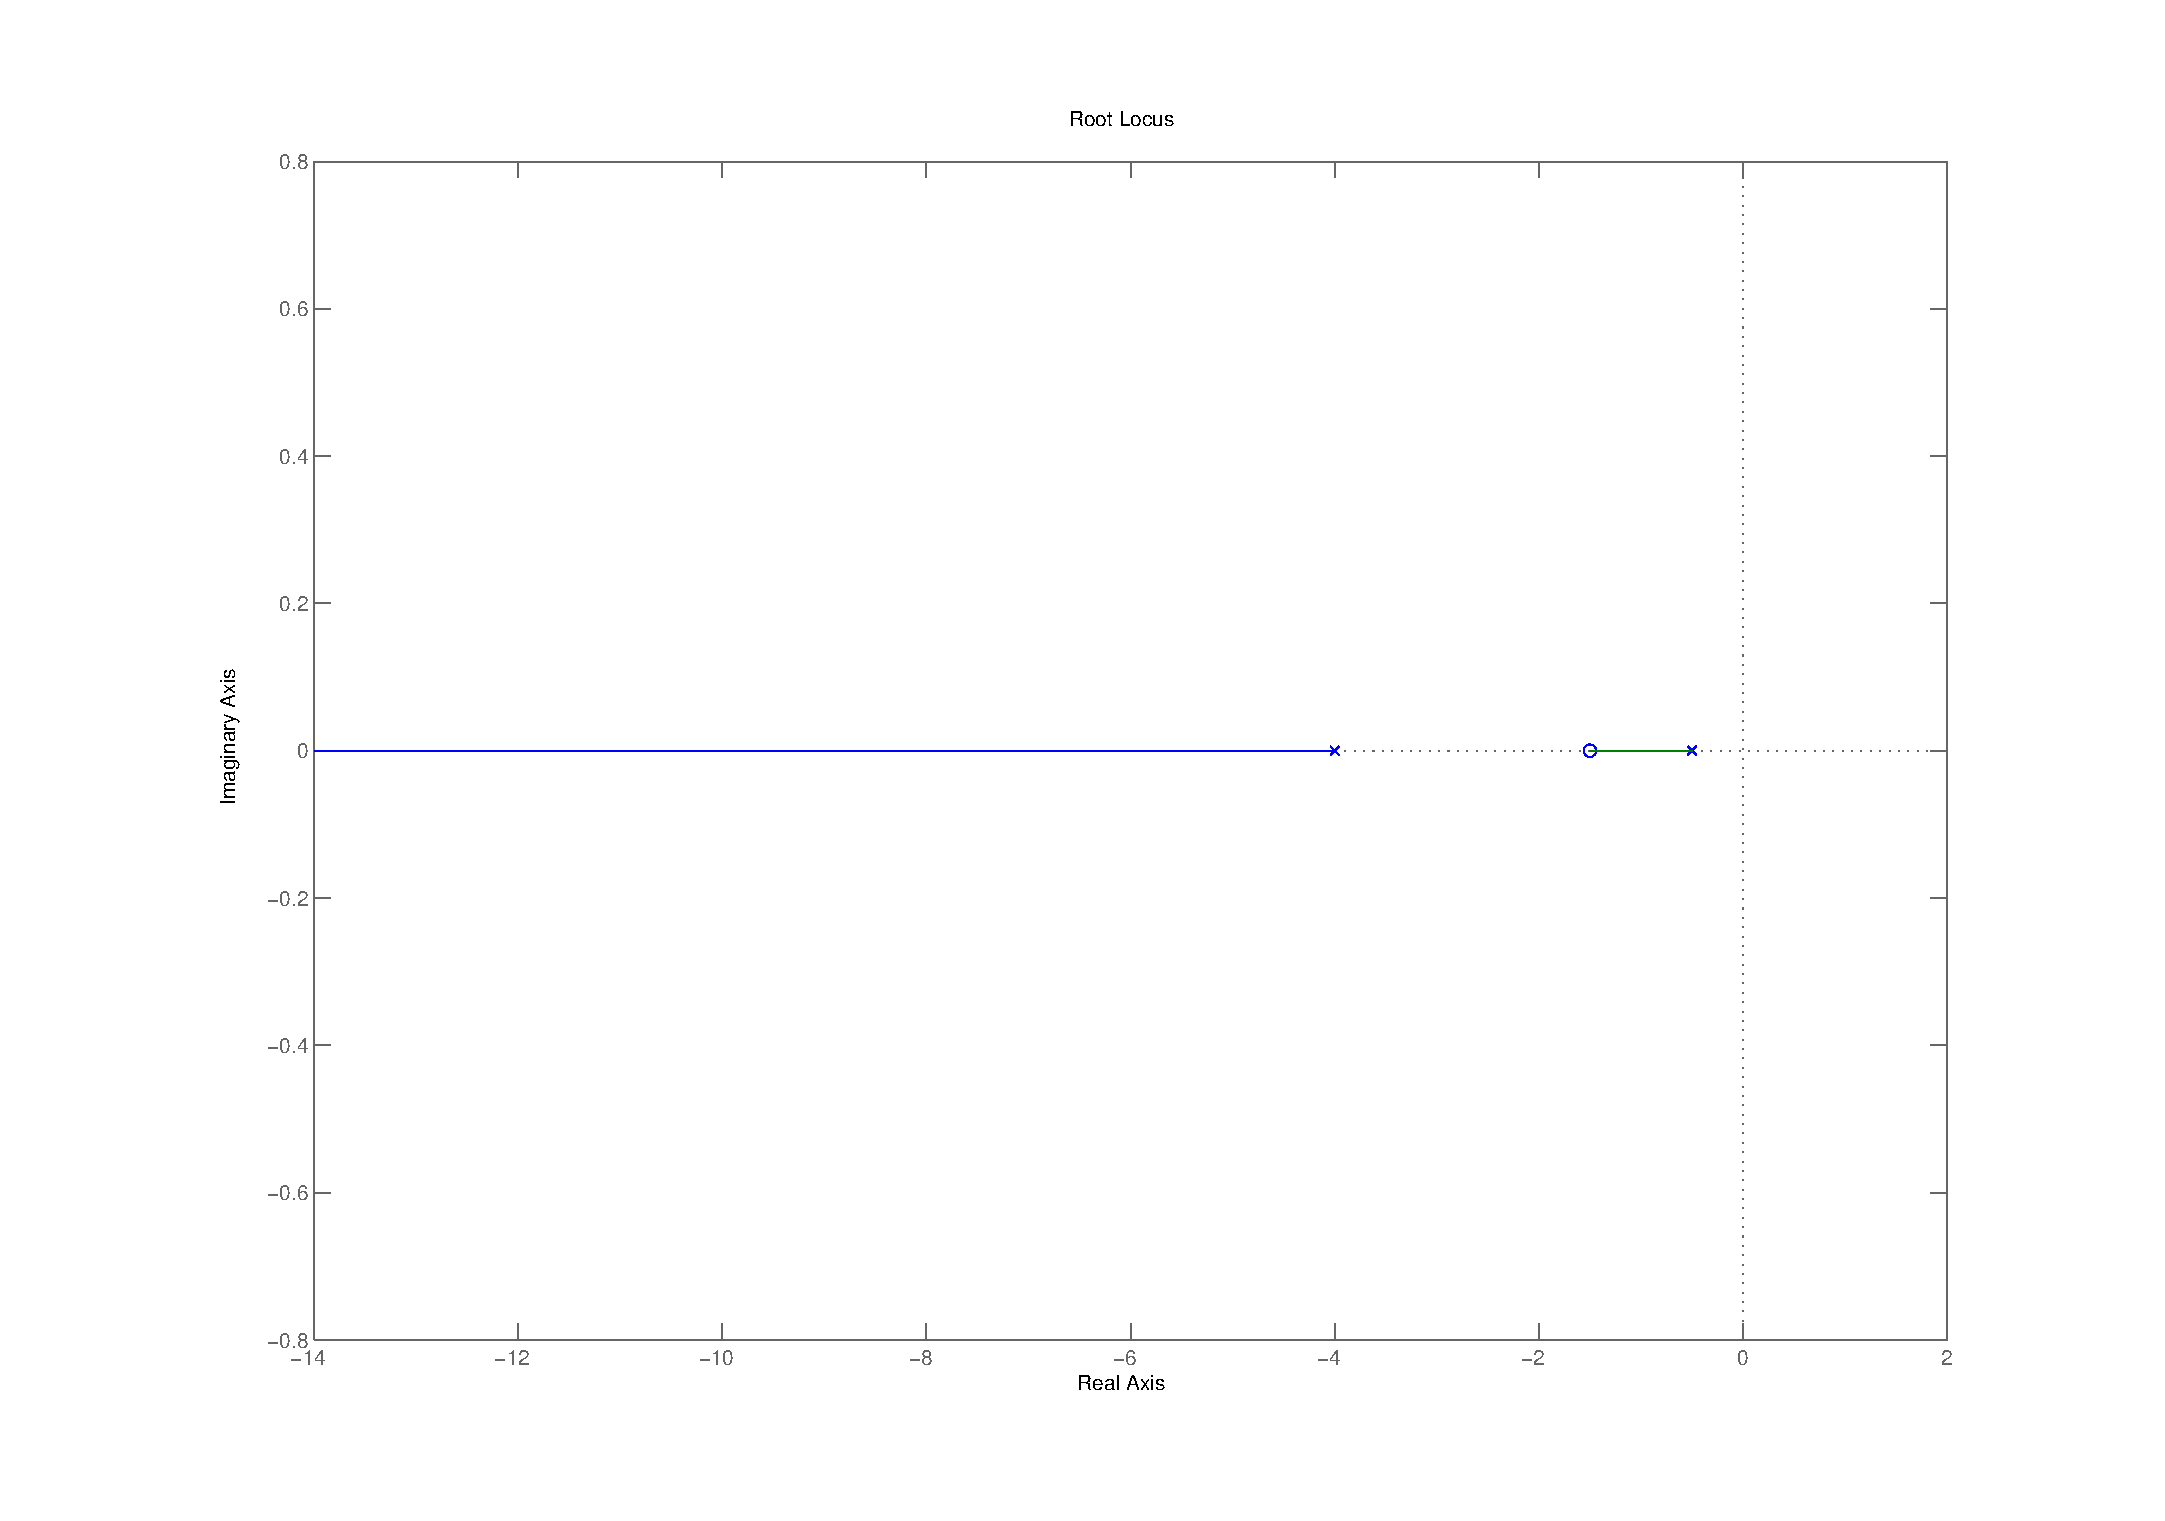
\includegraphics[width=0.8\textwidth]{imgs/questao2/rlocus_gma}
\caption{Lugar das raízes para os valores médios ($\vmedio{G}(s)$).}
\label{fig:q2:rlocus_gma}
\end{figure}

% TODO(crisgc): colocar diagrama de bloco com a malha fechada
Como um passo inicial, fechamos a malha e testamos a sua robustez segundo os
polinômios de Kharitonov. A função de transferência em malha fechada é mostrada a
seguir.

\begin{flalign}
G_{\text{MF}}(s) & = \frac{s+r}{(s+p)(s+q) + s+r} =
\frac{s+r}{s^{2}+\underbrace{(p+q+1)}_{a_1}s +
\underbrace{pq+r}_{a_0}} \nonumber \\
\vmedio{G_{\text{MF}}}(s) & = {\frac{1,5+s}{3,5+5,5s+s^{2}}} =
\frac{1,5+s}{(s+4,7656)(s+0,7344)} \quad
\bigtriangleup
\quad \text{Tomando os valores médios} \label{eq:q2:gmf}
\end{flalign}

Analisando a função de transferência de malha fechada, temos que:

\begin{flalign*}
a_0 &= pq+r & \alpha_0 & = \mymin{p}\mymin{q} + \mymin{r} = 1 \quad 
&\beta_0 &= \mymax{p}\mymax{q} + \mymax{r} = 7 \\
a_1 &= p + q + 1 & \alpha_1 &= \mymin{p} + \mymin{q} + 1 = 4 \quad
&\beta_1 &=\mymax{p} + \mymax{q} + 1 = 7
\end{flalign*}

Os quatro polinômios retirados do \textit{Teorema de Kharitonov} para o teste da
estabilidade são os seguintes:

\begin{flalign*}
q_0 & = \alpha_0 + \alpha_1s + s^{2} = 1 + 4s + s^{2} = (s + 3,7321)(s + 0,2679) \\ 
q_1 & = \alpha_0 + \beta_1s + s^{2} = 1 + 7s + s^{2} = (s + 6,8541)(s + 0,1459)\\ 
q_2 & = \beta_0 + \alpha_1s + s^{2} = 7 + 4s + s^{2} = (s + 2 + 1,7321i)(s + 2 -
1,7321i)\\ 
q_3 & = \beta_0 + \beta_1s + s^{2} = 7 + 7s + s^{2} = (s + 5,7913)(s + 1,2087)\\ 
\end{flalign*}

Logo como nenhum polo do sistema está situado no semiplano direito, ou seja,
todos os polos tem parte real negativa, o sistema é estável para qualquer valor
dos parâmetros dentro do seus intervalos de variação. Calculamos então o valor
final da resposta ao degrau unitário para avaliar seu valor no regime
permanente:

\begin{flalign*}
\lim_{t \tende \infty}{y(t)} & = \lim_{s \tende 0}sY(s) \\
Y(s) & = R(s)\vmedio{G_{\text{MF}}}(s) = \frac{1}{s}\frac{1,5+s}{3,5+5,5s+s^{2}} \\
\lim_{t \tende \infty}{y(t)} & =  \lim_{s \tende
0}s\frac{1}{s}\frac{1,5+s}{3,5+5,5s+s^{2}} = \frac{1,5}{3,5} = \frac{3}{7}
\approx 0,429
\end{flalign*}

\noindent o que condiz com o valor obtido por simulação (ver figura
\ref{fig:q2:resposta_gmf}).

\begin{figure}[htb]
\centering
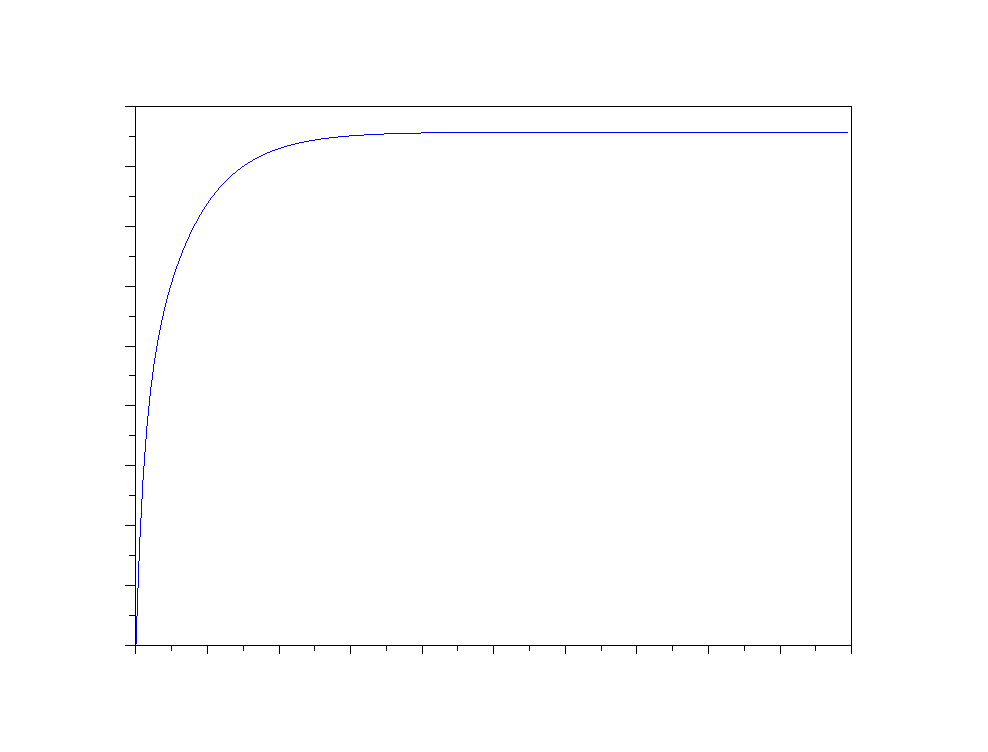
\includegraphics[width=0.8\textwidth]{imgs/questao2/resposta_gmf}
\caption{Resposta do sistema em malha fechada ao degrau unitário para um tempo de $20$s.}
\label{fig:q2:resposta_gma}
\end{figure}

O primeiro passo do projeto foi, então, um projeto de um controlador em atraso
de fase \cite{dorf:2009,maitelli2002} para a melhora do erro de regime a uma entrada
em degrau. A constante de erro de posição do sistema que obtivemos é dado por
$K_{p} = G(0) = 0,75$, o que resulta no erro de regime previamente calculado.
Decidimos adotar uma tolerância do erro de regime de aproximadamente  $1\%$ e
projetamos um compensador de modo que a constante de erro ficasse em $K'_p = 100$. O
controlador em atraso de fase tem a seguinte função de transferência:

% TODO(crisgc): Colocar a figura da resposta em malha fechada simples
\begin{flalign*}
G_c(s) & = k_c \frac{s+z_c}{s+p_c} \quad \text{onde} \quad |z_c| > |p_c| \\
\end{flalign*}

Portanto para obter a constante de erro desejada teríamos então que fazer:

\begin{flalign}
\underbrace{K'_{p}}_{100} & = G_c(0)G(0) = G_c(0)K_{p} = k_c \frac{z_c}{p_c}
\underbrace{K_{p}}_{0,75} \nonumber \\
k_c \frac{z_c}{p_c}& = \frac{100}{0,75} =  \frac{400}{3} \approx 133,333
\label{eq:q2:comp_atraso}
\end{flalign}

Como o polo dominante do sistema de malha aberta está localizado em $-0,5$ (ver
equação \ref{eq:q2:gma}) decidimos por alocar o zero do controlador à sua
direita, para que a interferência no regime transitório não seja muito
significante, fizemos então $z_c = 0,3$, optamos em um primeiro momento não
adicionar o ganho no controlador, portante fizemos $k_c = 1$. O polo, calculado
a partir de \ref{eq:q2:comp_atraso} foi então $p_c = 0,0022$. 

A função de transferência em malha fechada do sistema, $G_{\text{cMF}}$ (ver
figura \ref{fig:q2:malha_comp}) já com o controlador pode ser obtida através da
redução do diagrama de blocos e é mostrada a seguir:

\begin{figure}[htb]
\centering
\scalebox{0.7}{\input{imgs/questao2/compensador_malha.pstex_t}}
\caption{Diagrama de blocos para o sistema com o compensador.}
\label{fig:q2:malha_comp}
\end{figure}

\begin{flalign}
G_\text{cMF}(s) & = \frac{G_c(s)G(s)}{1 + G_c(s)G(s)} =
\frac{k_c(s+z_c)(s+r)}{k_c(s+z_c)(s+r) + (s+p)(s+q)(s+p_c)} \nonumber \\
& = \frac{k_cs^{2} + k_c(z_c + r)s + k_crz_c}{s^{3} + \underbrace{[k_c + p_c +
(p+q)]}_{a_2}s^{2} +
\underbrace{[k_c(r+z_c) + p_c(p+q)+pq]}_{a_1}s + \underbrace{rz_c + pqp_c}_{a_0}
} \label{eq:q2:testeKharitonov}
\end{flalign}

Testamos a estabilidade do sistema segundo o \textit{teorema de Kharitonov}
utilizando o o script mostrado no apêndice \ref{ap:q2:testeKharitonov}.
Os quatro polinômio para os valores calculador do controlador, a saber $z_c = 0,3$, $k_c 
= 1$ e $p_c = 0,0022$, são os seguintes:

\begin{flalign*}
q_1 & = 0,3+1,3066s+7,0022s^{2}+s^{3} \\
q_2 & = 0,3+7,3132s+7,0022s^{2}+s^{3} \\
q_3 & = 0,611+1,3066s+5,0022s^{2}+s^{3} \\
q_4 & = 0,611+7,3132s+5,0022s^{2}+s^{3}
\end{flalign*}

\noindent e os polos de cada um desses polinômios podem ser visualizados na
seguinte matriz, onde cada coluna é referente a um polinômio. 

\begin{flalign*}
\begin{pmatrix}-0,093+0,188i&-0,043&-0,124+0,336i&-0,089\cr
-0,093-0,188i&-1,223&-0,124-0,336i&-2,457+0,917i\cr
-6,817&-5,736&-4,754&-2,457-0,917i\cr \end{pmatrix}
\end{flalign*}

\noindent logo podemos ver que o controlador desenvolvido é robusto para a faixa
estabelecida de variação dos parâmetros. E o resultado da resposta ao degrau com
o controlador pode ser visualizada na figura \ref{fig:q2:resposta_gcomp1}.
Através da análise da figura podemos ver que embora o desempenho do regime
permanente tende para o valor desejado (próximo a 1), a demora do sistema na
subida pode ser um problema que precisa ser evitado.
 
\begin{figure}[htb]
\centering
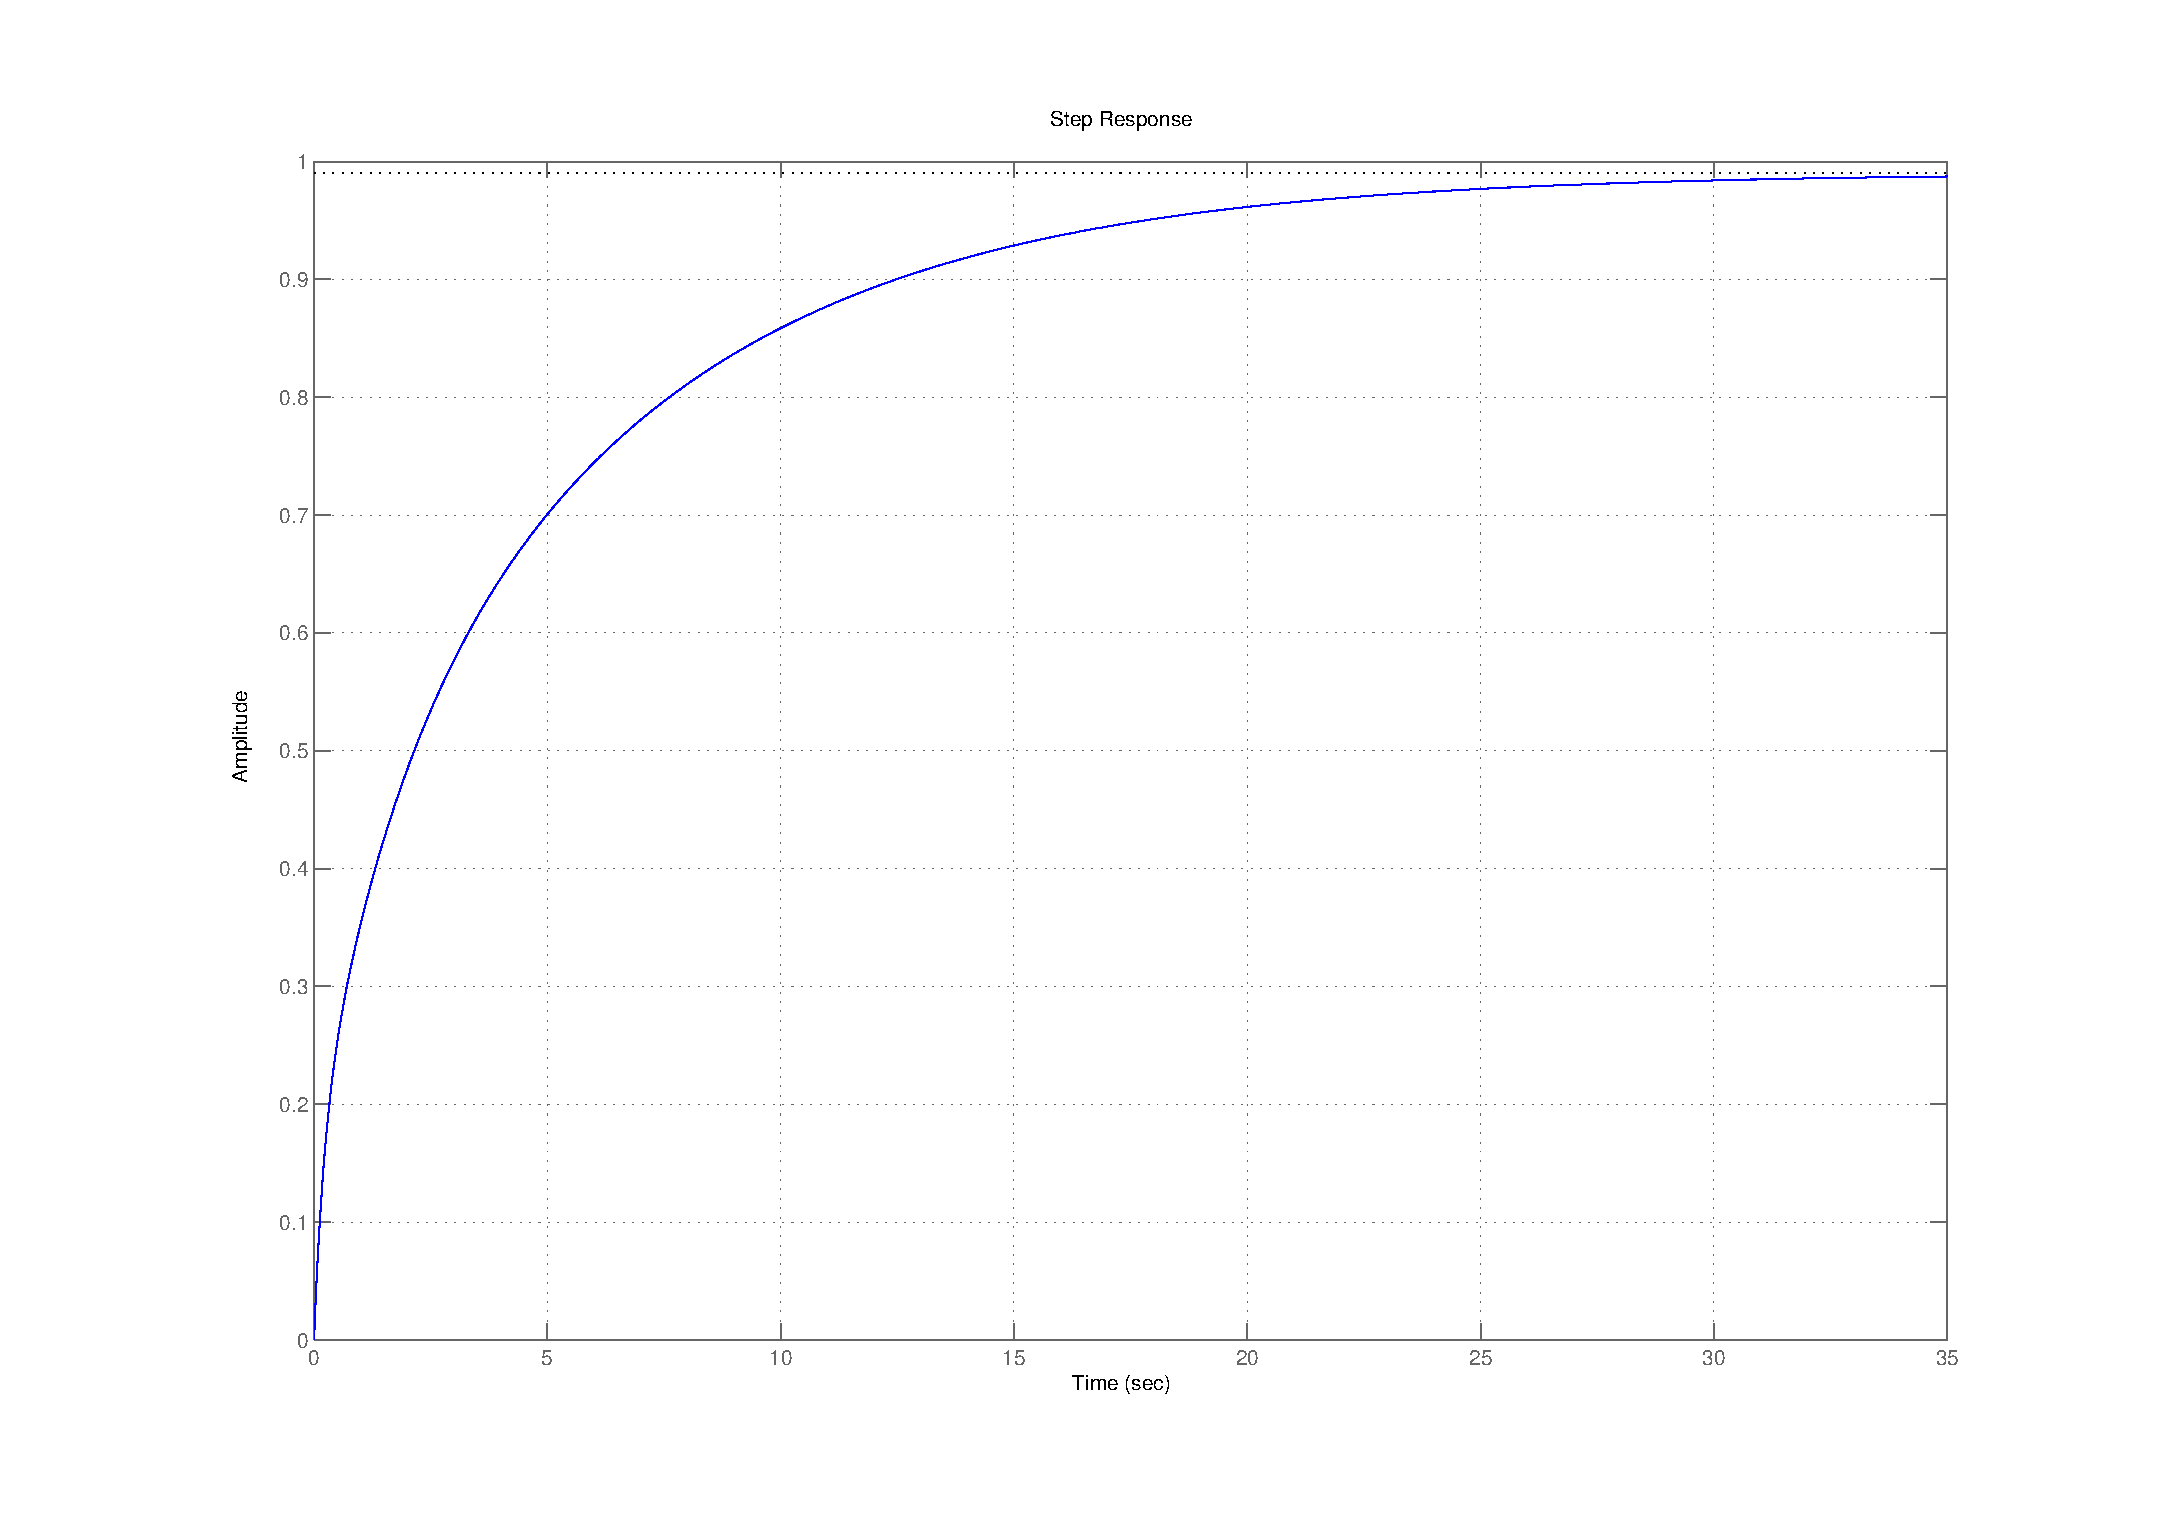
\includegraphics[width=0.8\textwidth]{imgs/questao2/resposta_gcomp1}
\caption{Resposta ao degrau para o controlador $G_c(s) = \frac{s+0,3}{s+0,0022}$}
\label{fig:q2:resposta_gcomp1}
\end{figure}

Então, para evitar esse problema, analisamos mais o lugar das raízes do sistema
em malha aberta com o controlador (ver figura \ref{fig:q2:rlocus_gcomp1}), e,
para melhorar o desempenho do tempo de subida decidimos por aumentar o ganho do
sistema, distanciando, dessa forma, os polos do eixo imaginário, dessa forma
tornando o sistema mais rápido. Testamos com um ganho para o controlador $k_c =
20$ e obtivemos, a resposta para o sistema em malha fechada mostrada na figura
\ref{fig:q2:resposta_gcomp2}.

\begin{figure}[htb]
\centering
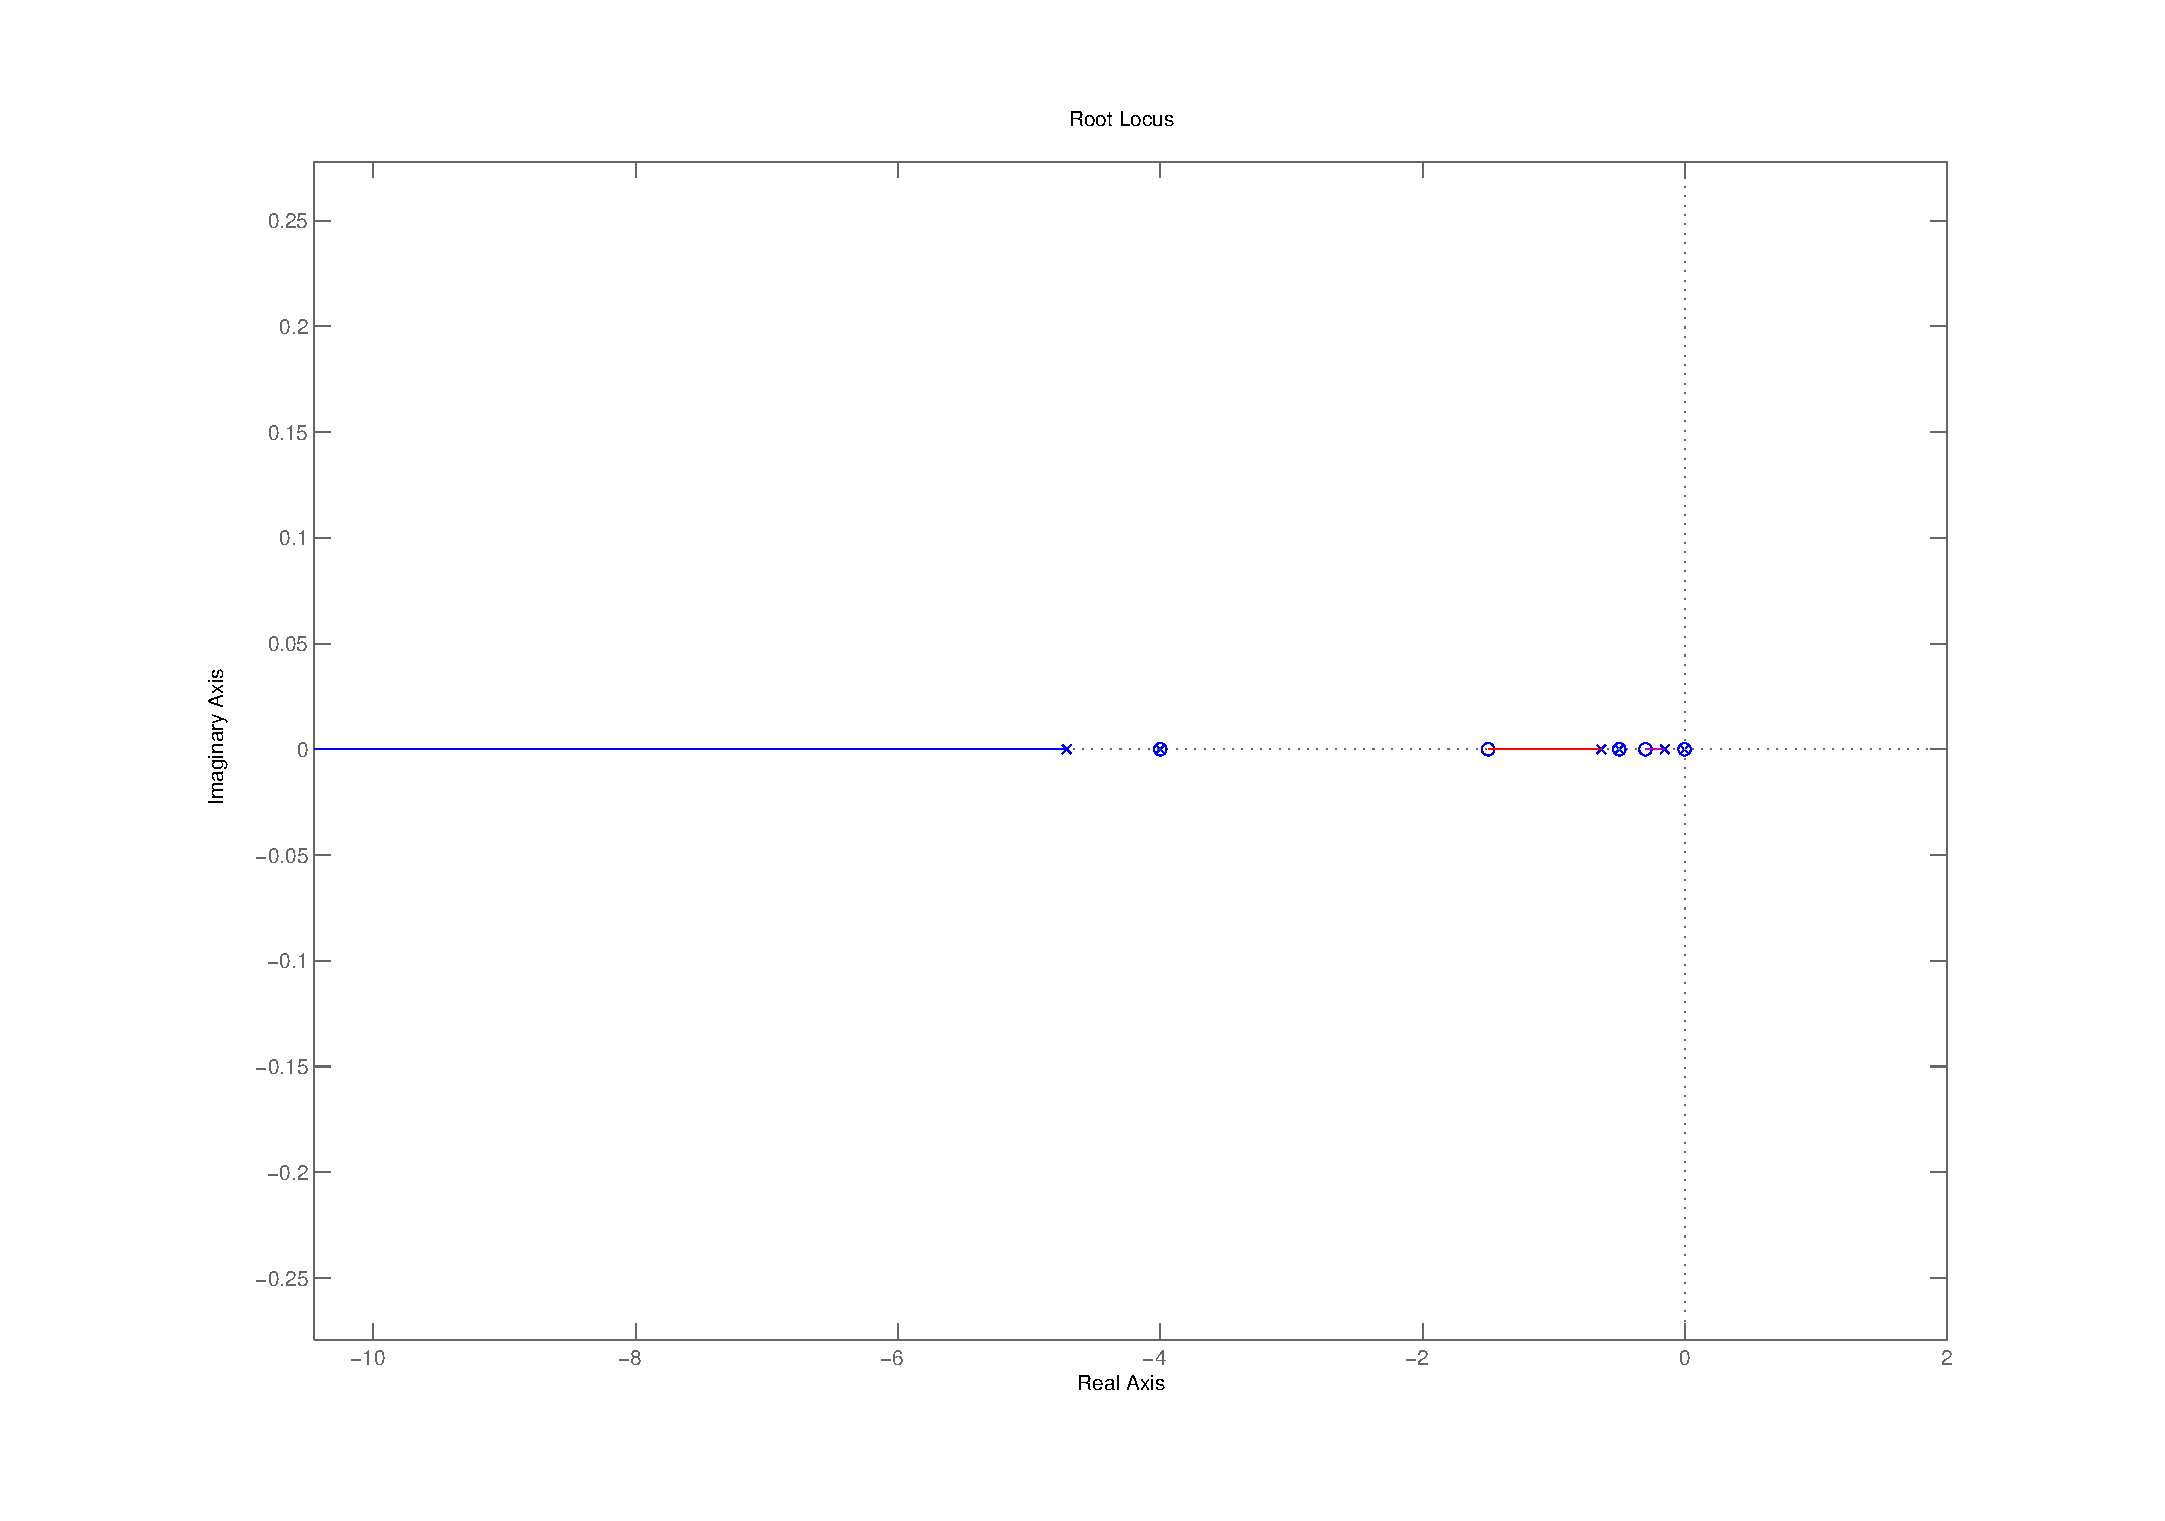
\includegraphics[width=0.8\textwidth]{imgs/questao2/rlocus_gcma}
\caption{Lugar das raízes para o sistema com o controlador $G_c(s)$}
\label{fig:q2:rlocus_gcomp1}
\end{figure}
 
\begin{figure}[H]
\centering
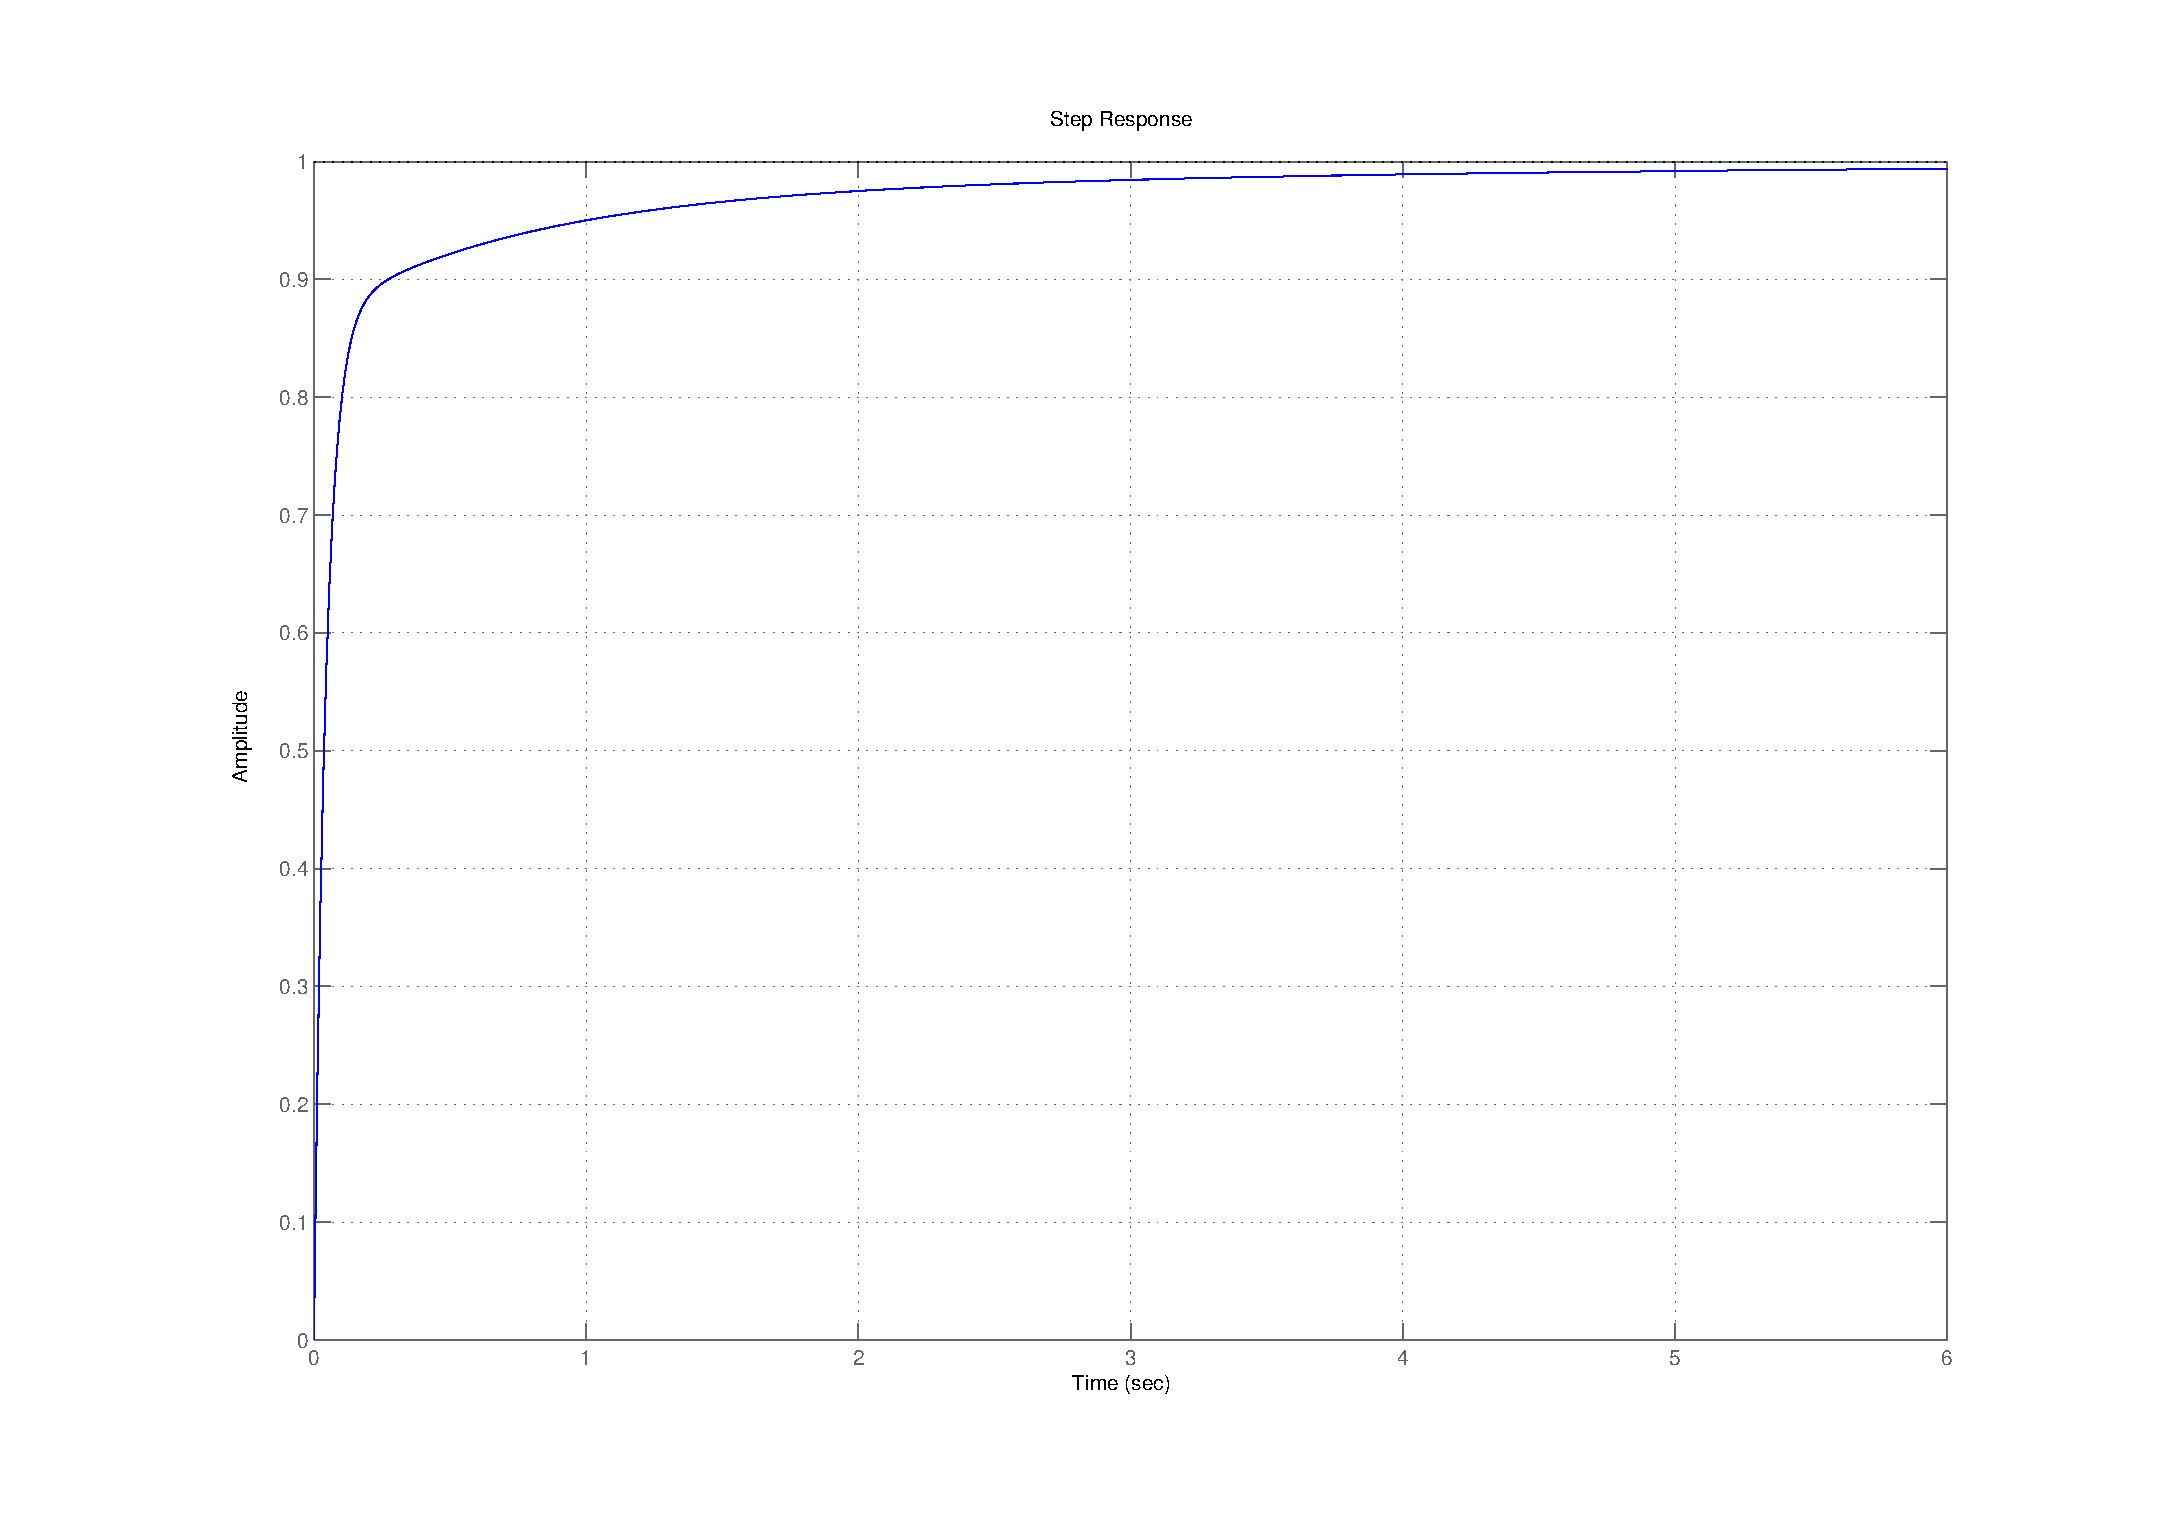
\includegraphics[width=0.8\textwidth]{imgs/questao2/resposta_gcomp2}
\caption{Reposta do sistema com o controlador $G_c(s) = 20\frac{s+0,3}{s+0,0022}$ }
\label{fig:q2:resposta_gcomp2}
\end{figure}

Podemos visualizar a melhora substancial no tempo de subida do sistema. Testamos
então a estabilidade do sistema para a faixa de variação de parâmetros mais uma
vez através dos polinômios de Kharitonov (ver equação
\ref{eq:q2:testeKharitonov} e o apêndice \label{ap:q2:testeKharitonov}) e
obtivemos os seguintes polinômios:

\begin{flalign*}
q_1 & = 0.3+26.0066s+26.0022s^{2}+s^{3} \\
q_2 & = 0.3+51.0132s+26.0022s^{2}+s^{3} \\
q_3 & = 0.611+26.0066s+24.0022s^{2}+s^{3} \\
q_4 & = 0.611+51.0132s+24.0022s^{2}+s^{3}
\end{flalign*}

\noindent e as suas raízes:

\begin{flalign*}
\begin{pmatrix}-0.012&-0.006&-0.024&-0.012\cr -1.03&-2.131&-1.112&-2.343\cr
-24.961&-23.865&-22.866&-21.647\cr \end{pmatrix}
\end{flalign*}

O sistema é estável na faixa de variação dada dos parâmetros de $G(s)$. Logo o
controle é robusto. Como a resposta em regime permanente como em
regime transitório é satisfatória, o controlador em atraso de fase foi
suficiente para o projeto do sistema, e a parte em avanço de fase não foi
projetada. O controlador projetado é portanto:

\begin{flalign*}
G_c(s) = 20\frac{s+0,3}{s+0,0022}
\end{flalign*}

% TODO(crisgc): Colocar o desempenho do controlador para alguns valores
% "randômicos" da função de transferência
